%===============================================================================
% LaTeX sjabloon voor de bachelorproef toegepaste informatica aan HOGENT
% Meer info op https://github.com/HoGentTIN/bachproef-latex-sjabloon
%===============================================================================

\documentclass{bachproef-tin}

\usepackage{hogent-thesis-titlepage} % Titelpagina conform aan HOGENT huisstijl

%%---------- Documenteigenschappen ---------------------------------------------
% TODO: Vul dit aan met je eigen info:

% De titel van het rapport/bachelorproef
\title{Titel}

% Je eigen naam
\author{Steven Stevens}

% De naam van je promotor (lector van de opleiding)
\promotor{Jan Janssens}

% De naam van je co-promotor. Als je promotor ook je opdrachtgever is en je
% dus ook inhoudelijk begeleidt (en enkel dan!), mag je dit leeg laten.
\copromotor{Piet Pieters}

% Indien je bachelorproef in opdracht van/in samenwerking met een bedrijf of
% externe organisatie geschreven is, geef je hier de naam. Zoniet laat je dit
% zoals het is.
\instelling{---}

% Academiejaar
\academiejaar{2018-2019}

% Examenperiode
%  - 1e semester = 1e examenperiode => 1
%  - 2e semester = 2e examenperiode => 2
%  - tweede zit  = 3e examenperiode => 3
\examenperiode{2}

%===============================================================================
% Inhoud document
%===============================================================================

\begin{document}

%---------- Taalselectie -------------------------------------------------------
% Als je je bachelorproef in het Engels schrijft, haal dan onderstaande regel
% uit commentaar. Let op: de tekst op de voorkaft blijft in het Nederlands, en
% dat is ook de bedoeling!

%\selectlanguage{english}

%---------- Titelblad ----------------------------------------------------------
\inserttitlepage

%---------- Samenvatting, voorwoord --------------------------------------------
\usechapterimagefalse
%%=============================================================================
%% Voorwoord
%%=============================================================================

\chapter*{\IfLanguageName{dutch}{Woord vooraf}{Preface}}
\label{ch:voorwoord}

%% TODO:
%% Het voorwoord is het enige deel van de bachelorproef waar je vanuit je
%% eigen standpunt (``ik-vorm'') mag schrijven. Je kan hier bv. motiveren
%% waarom jij het onderwerp wil bespreken.
%% Vergeet ook niet te bedanken wie je geholpen/gesteund/... heeft


%%=============================================================================
%% Samenvatting
%%=============================================================================

% TODO: De "abstract" of samenvatting is een kernachtige (~ 1 blz. voor een
% thesis) synthese van het document.
%
% Deze aspecten moeten zeker aan bod komen:
% - Context: waarom is dit werk belangrijk?
% - Nood: waarom moest dit onderzocht worden?
% - Taak: wat heb je precies gedaan?
% - Object: wat staat in dit document geschreven?
% - Resultaat: wat was het resultaat?
% - Conclusie: wat is/zijn de belangrijkste conclusie(s)?
% - Perspectief: blijven er nog vragen open die in de toekomst nog kunnen
%    onderzocht worden? Wat is een mogelijk vervolg voor jouw onderzoek?
%
% LET OP! Een samenvatting is GEEN voorwoord!

%%---------- Nederlandse samenvatting -----------------------------------------
%
% TODO: Als je je bachelorproef in het Engels schrijft, moet je eerst een
% Nederlandse samenvatting invoegen. Haal daarvoor onderstaande code uit
% commentaar.
% Wie zijn bachelorproef in het Nederlands schrijft, kan dit negeren, de inhoud
% wordt niet in het document ingevoegd.

\IfLanguageName{english}{%
\selectlanguage{dutch}
\chapter*{Samenvatting}
\lipsum[1-4]
\selectlanguage{english}
}{}

%%---------- Samenvatting -----------------------------------------------------
% De samenvatting in de hoofdtaal van het document

\chapter*{\IfLanguageName{dutch}{Samenvatting}{Abstract}}

\lipsum[1-4]


%---------- Inhoudstafel -------------------------------------------------------
\pagestyle{empty} % Geen hoofding
\tableofcontents  % Voeg de inhoudstafel toe
\cleardoublepage  % Zorg dat volgende hoofstuk op een oneven pagina begint
\pagestyle{fancy} % Zet hoofding opnieuw aan

%---------- Lijst figuren, afkortingen, ... ------------------------------------

% Indien gewenst kan je hier een lijst van figuren/tabellen opgeven. Geef in
% dat geval je figuren/tabellen altijd een korte beschrijving:
%
%  \caption[korte beschrijving]{uitgebreide beschrijving}
%
% De korte beschrijving wordt gebruikt voor deze lijst, de uitgebreide staat bij
% de figuur of tabel zelf.

\listoffigures
\listoftables

% Als je een lijst van afkortingen of termen wil toevoegen, dan hoort die
% hier thuis. Gebruik bijvoorbeeld de ``glossaries'' package.
% https://www.overleaf.com/learn/latex/Glossaries

%---------- Kern ---------------------------------------------------------------

% De eerste hoofdstukken van een bachelorproef zijn meestal een inleiding op
% het onderwerp, literatuurstudie en verantwoording methodologie.
% Aarzel niet om een meer beschrijvende titel aan deze hoofstukken te geven of
% om bijvoorbeeld de inleiding en/of stand van zaken over meerdere hoofdstukken
% te verspreiden!

%%=============================================================================
%% Inleiding
%%=============================================================================

\chapter{\IfLanguageName{dutch}{Inleiding}{Introduction}}
\label{ch:inleiding}

De inleiding moet de lezer net genoeg informatie verschaffen om het onderwerp te begrijpen en in te zien waarom de onderzoeksvraag de moeite waard is om te onderzoeken. In de inleiding ga je literatuurverwijzingen beperken, zodat de tekst vlot leesbaar blijft. Je kan de inleiding verder onderverdelen in secties als dit de tekst verduidelijkt. Zaken die aan bod kunnen komen in de inleiding~\autocite{Pollefliet2011}:

\begin{itemize}
  \item context, achtergrond
  \item afbakenen van het onderwerp
  \item verantwoording van het onderwerp, methodologie
  \item probleemstelling
  \item onderzoeksdoelstelling
  \item onderzoeksvraag
  \item \ldots
\end{itemize}

\section{\IfLanguageName{dutch}{Probleemstelling}{Problem Statement}}
\label{sec:probleemstelling}

Uit je probleemstelling moet duidelijk zijn dat je onderzoek een meerwaarde heeft voor een concrete doelgroep. De doelgroep moet goed gedefinieerd en afgelijnd zijn. Doelgroepen als ``bedrijven,'' ``KMO's,'' systeembeheerders, enz.~zijn nog te vaag. Als je een lijstje kan maken van de personen/organisaties die een meerwaarde zullen vinden in deze bachelorproef (dit is eigenlijk je steekproefkader), dan is dat een indicatie dat de doelgroep goed gedefinieerd is. Dit kan een enkel bedrijf zijn of zelfs één persoon (je co-promotor/opdrachtgever).

\section{\IfLanguageName{dutch}{Onderzoeksvraag}{Research question}}
\label{sec:onderzoeksvraag}

Wees zo concreet mogelijk bij het formuleren van je onderzoeksvraag. Een onderzoeksvraag is trouwens iets waar nog niemand op dit moment een antwoord heeft (voor zover je kan nagaan). Het opzoeken van bestaande informatie (bv. ``welke tools bestaan er voor deze toepassing?'') is dus geen onderzoeksvraag. Je kan de onderzoeksvraag verder specifiëren in deelvragen. Bv.~als je onderzoek gaat over performantiemetingen, dan 

\section{\IfLanguageName{dutch}{Onderzoeksdoelstelling}{Research objective}}
\label{sec:onderzoeksdoelstelling}

Wat is het beoogde resultaat van je bachelorproef? Wat zijn de criteria voor succes? Beschrijf die zo concreet mogelijk. Gaat het bv. om een proof-of-concept, een prototype, een verslag met aanbevelingen, een vergelijkende studie, enz.

\section{\IfLanguageName{dutch}{Opzet van deze bachelorproef}{Structure of this bachelor thesis}}
\label{sec:opzet-bachelorproef}

% Het is gebruikelijk aan het einde van de inleiding een overzicht te
% geven van de opbouw van de rest van de tekst. Deze sectie bevat al een aanzet
% die je kan aanvullen/aanpassen in functie van je eigen tekst.

De rest van deze bachelorproef is als volgt opgebouwd:

In Hoofdstuk~\ref{ch:stand-van-zaken} wordt een overzicht gegeven van de stand van zaken binnen het onderzoeksdomein, op basis van een literatuurstudie.

In Hoofdstuk~\ref{ch:methodologie} wordt de methodologie toegelicht en worden de gebruikte onderzoekstechnieken besproken om een antwoord te kunnen formuleren op de onderzoeksvragen.

% TODO: Vul hier aan voor je eigen hoofstukken, één of twee zinnen per hoofdstuk

In Hoofdstuk~\ref{ch:conclusie}, tenslotte, wordt de conclusie gegeven en een antwoord geformuleerd op de onderzoeksvragen. Daarbij wordt ook een aanzet gegeven voor toekomstig onderzoek binnen dit domein.
\chapter{\IfLanguageName{dutch}{Stand van zaken}{State of the art}}
\label{ch:stand-van-zaken}

% Tip: Begin elk hoofdstuk met een paragraaf inleiding die beschrijft hoe
% dit hoofdstuk past binnen het geheel van de bachelorproef. Geef in het
% bijzonder aan wat de link is met het vorige en volgende hoofdstuk.
Bedrijven zijn constant op zoek naar betere en snellere resultaten. In het software development circuit is het vandaag soms nog lang wachten voor een wijziging effectief doorgevoerd wordt. Men levert nog vaak software op aan het einde van de sprint, wat soms voor problemen zorgt als men veel code tegelijk aflevert. Met een nieuwe software development methode - Continuous Integration en Continuous Delivery genaamd - wil men deze problemen zoveel mogelijk vermijden. Er wordt vaak gesproken van een CI/CD pipeline als het gaat over Continuous Integration en Continuous Delivery, maar er is nog een derde speler dat men kan invoeren: Continuous Deployment. Samen vormen zij de 3 musketiers om software projecten een grotere slaagkans te geven.
Om een duidelijker beeld te scheppen van een CI/CD pipeline zal dit hoofdstuk eerst uitleg verschaffen over DevOps, Continuous Integration, Continuous Delivery en Continuous Deployment. Daarna wordt er kort in detail gegaan hoe het bedrijf Amista eruit ziet en met welke tools ze werken. Tot slot wordt er uitgelegd hoe de grote structuur van een CI/CD pipeline eruit ziet.

% Pas na deze inleidende paragraaf komt de eerste sectiehoofding.

\section{Continuous Integration, Continuous Delivery \& Continuous Deployment}
\label{sec:continuous-integration-continuous-delivery-continuous-deployment}
    \paragraph{DevOps}
    DevOps is een samentrekking van development en operations en is een welbekend begrip binnen de informatica wereld. Het heeft als doel om de 'state of mind' binnen een bedrijf te veranderen zodat alle lagen/departementen vlotter samenwerken. Het is een praktische 'gids' dat bedrijven kunnen gebruiken om de communicatie tussen developers en systeembeheerders beter te maken. Deze twee verschillende lagen in een bedrijf willen namelijk hetzelfde: zo snel mogelijk kwaliteitsvolle software opleveren. DevOps is gebaseerd op Agile development, maar gaat verder dan dat. Het gaat dieper in op automatisatie, integratie, samenwerking en communicatie. 
    Continuous Integration, Delivery en Deployment zijn kenmerkend voor DevOps, omdat het mee inzet op snellere oplevering van kwaliteitsvolle software. ~\autocite{Riti2018}
    
    % Hier zeker Patrick Debois vernoemen en vermelden waarom DevOps is opgericht: omdat ze in 2008 veel te maken hadden met falende projecten vanwege slechte communicatie.

    \paragraph{Continuous Integration}
    Dit is een eerste stap in de pipeline waarbij de geschreven code wordt gecommit naar een 'repository management server'. Hierdoor wordt de 'source code' automatisch opnieuw opgebouwd en slaagt voor de testen die automatisch zijn opgestart. De focus bij deze stap ligt bij de teamleden ~\autocite{Fowler2006}, van hen wordt verwacht dat ze - op regelmatige basis - hun code pushen (integreren met de master applicatie). Een goede samenwerking tussen de verschillende leden van het development team is broodnodig om tot het gewenste eindresultaat te komen.
    Het doel van een Continuous Integration is om de integratie feilloos te laten verlopen wanneer men software ontwikkelt en geen functionaliteiten verliezen na een merge ~\autocite{Riti2018}.
    \newline
    Bovenstaande uitleg is makkelijker te begrijpen aan de hand van een voorbeeld. Op Figuur \ref{img-ci-example} is een grafische voorstelling van dit voorbeeld terug te vinden.
    De developer maakt een wijziging en commit de code naar de repository die te vinden is op het source-control systeem. De Continuous Integration server krijgt het bericht dat er code is toegevoegd, haalt de laatst toegevoegde code op en laat de testen runnen. Wanneer alle testen slagen zal de CI server de code compilen en feedback bezorgen aan de developer. In dit voorbeeld maakt men gebruik van een externe mail server om die feedback te verzenden.
    Deze stappen gebeuren elke keer er code naar de repository gestuurd wordt.
    Bovenstaand voorbeeld is een best-practice hoe het zou moeten gebeuren. Er zijn echter enkele zaken die wat extra uitleg kunnen gebruiken.
    De frequentie en hoeveelheid code zijn belangrijke zaken waar de developer rekening mee moet houden bij een CI pipeline. Volgens \textcite{Fowler2006} is het de plicht van een developer om minstens 1 maal per dag een commit te doen. Hij moet telkens een commit uitvoeren wanneer hij een kleine opdracht afgerond heeft. Zo blijft de hoeveelheid code klein en is het makkelijk om te zoeken wanneer er zich een probleem voordoet.
    Eens de wijziging gecommit is naar de version control repository moet de CI pipeline zijn werk doen. Een belangrijke stap is het bezorgen van de feedback. Dit moet namelijk het resultaat van de build en de feedback waar het probleem zich kan bevinden terug geven, door bijvoorbeeld aan te geven welke test niet slaagt bij het uitvoeren van de automated testing. De key factor hier is de tijd. Als de developer pas daags nadien feedback krijgt over de fout die hij gepusht heeft, wordt het al moeilijker om de fout te vinden en ze op te lossen. 
    \begin{figure}	
        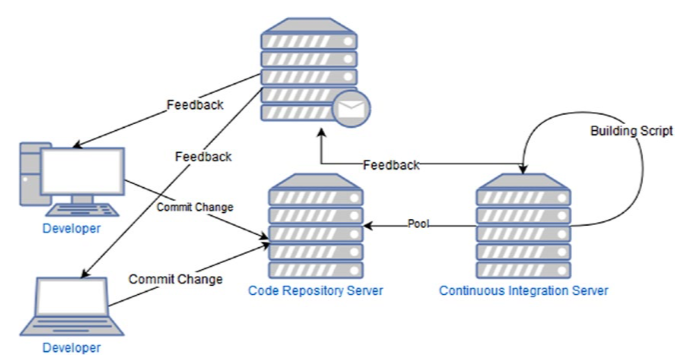
\includegraphics[scale=0.65]{ci-example}
        \caption{Voorbeeld van een Continuous Integration set-up ~\autocite{Riti2018}} \label{img-ci-example}
    \end{figure}

    \paragraph{Continuous Delivery}
    Eens het team met succes de Continuous Integration toepast kan men overschakelen naar de volgende stap: Continuous Delivery.
    Het is een manier dat ervoor zorgt dat de code die van de Continuous Integration stap komt, gebuild en voorbereid wordt voor een release.
    Er is echter wel nog een menselijke hand nodig om de build van deze stap te deployen en voor de buitenwereld beschikbaar te stellen ~\autocite{Fowler2013}.
    \newline{}In Figuur \ref{img-cd-chain} ziet men hoe een Continuous Delivery chain is opgebouwd, het is een grafische weergave van de stappen die een Continuous Delivery pipeline moet hebben. Dit is gebaseerd op de Continuous Integration chain, maar hier zijn extra stappen toegevoegd.
    De eerste stap is het developen van de code die men wenst op te leveren. Net zoals bij Continuous Integration commit de developer de code naar de version control repository. De build scheduler haalt de laatst toegevoegde code op en test deze code. Enkel bij het slagen van alle testen wordt de code gebuild door de build scheduler. Deze maakt ook de build klaar voor release en vereist enkel nog menselijke goedkeuring om deze release te lanceren.
    \newline{}In dit proces is feedback ook uiterst belangrijk. Als men foute code pusht, moet de persoon die deze code geschreven heeft zo snel mogelijk verwittigd worden. Op deze manier kan het euvel snel opgelost worden.
    Mail kan een vorm zijn van feedback, maar er bestaan nog andere leuke vormen naast mailing. Het bedrijf Dynatrace heeft bijvoorbeeld een licht ontworpen dat je in de kamer van het team kan hangen. Dit Internet of Things (IoT) gadget, DevOps UFO genaamd, is via WiFi verbonden aan de pipeline omgeving. Het geeft feedback over de staat van de CI/CD pipeline en is een vorm van monitoring. Het geeft de developers en iedereen in de kamer onmiddelijke feedback wanneer er een commit gebeurd. Als de commit door de pipeline geraakt zal de UFO groen kleuren, wanneer de build faalt kleurt de UFO rood en weet iedereen dat er een fout is. Zo weet de persoon die de foute code gepusht heeft dat er iets fout is en kan hij hier nog sneller op inspelen. 
    \begin{figure}	
        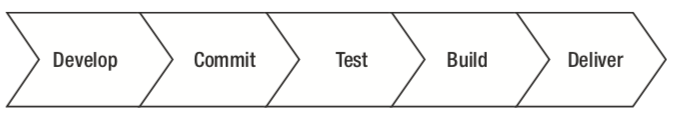
\includegraphics[scale=0.65]{cd-chain}
        \caption{Continuous Delivery chain ~\autocite{Riti2018}} \label{img-cd-chain}
    \end{figure}
    
    \paragraph{Continuous Deployment}
    De gelijkenis met Continuous Deployment is treffend, maar er is wel degelijk een verschil.
    Hier gaat men automatisch de veranderde code naar productie brengen. De veranderingen gaan door de volledige pipeline en eens ze slagen voor alle testen wordt - zonder menselijke interactie - de code naar productie gebracht ~\autocite{Claps2015}.
    Dit wordt soms ook wel de 'train to production' genoemd, omdat elke code dat gepusht wordt naar de source-control automatisch tot bij de klant geraakt.
    
    \paragraph{Automated Testing}
    Zoals hierboven reeds aangegeven is er geen Continuous Integration pipeline zonder automated testing. Het grootste doel van deze fase is - zoals de naam het zegt - testen van de code. Als de CI/CD pipeline voorzien wordt van voldoende en goede testen, wordt er een veiligheidsgevoel gecreëerd. Men is zeker dat de software aan bepaalde criteria voldoet, die in de testen verwerkt worden. Het is dus een heel belangrijk onderdeel van de pipeline waar veel aandacht aan besteed moet worden. 
    Om te voldoen aan de criteria van CI/CD moeten de testen automatisch gerund worden. Dit was tot voor kort echter vaak niet het geval. Er waren testers aangesteld om telkens opnieuw software te testen, door op de verschillende knoppen te drukken in de user interface (UI). Heel vaak slopen er fouten in omdat dit heel repetitief en saai werk was. Daar komt de automated van pas, dit zorgt ervoor dat alles automatisch gebeurd ~\autocite{Vocke2018}.
    \newline{}
    %TODO: Test pyramid uitleggen en verwijzen naar figuur! https://martinfowler.com/articles/practical-test-pyramid.html
    %Mike Cohn kwam met het idee om testen op te delen in drie grote categorieën: Unit Tests, Service Tests en UI tests. 
    Om ervoor te zorgen dat de automated tests de noden van Continuous Integration behagen zijn er bepaalde criteria.
    Wanneer men de testen schrijft moet men rekening houden met snelheid, betrouwbaarheid, hoeveelheid en onderhoud.
    %TODO: Guide-To-Devops-2019 pagina 16 staat uitleg dat ik hier nog moet schrijven
    

\section{SAP}
\label{sec:sap}
    SAP is een Duitse onderneming opgericht in 1972 dat softwareoplossingen aanbiedt voor grote ondernemingen. Met meer dan 413.000 klanten verspreid over 180 landen mag SAP zich marktleider noemen op gebied van bedrijfssoftware.
    SAP heeft zicht gespecialiseerd in ERP, Enterprise Resource Planning software dat alle processen van het bedrijf automatiseert ~\autocite{SAPERP2019}. Een ERP systeem beheert meerdere functies en bedrijfsprocessen van één bedrijf op basis van een centrale database. Het heeft als doel de gegevens van de organisatie optimaal te gebruiken in de gehele organisatie en een betere beheersing van de bedrijfsprocessen voorzien.
    De oplossingen die SAP aanbiedt zijn vooral bedoeld voor de grotere bedrijven. Ze bieden software aan voor elke mogelijke industrie die er vandaag de dag bestaat, maar pakken uit met hun specialiteiten in de cloud business software.
    Hieronder worden kort de programma's beschreven die gebruikt worden in de voorbeeldapplicatie. Het geeft een grof beeld van de omgeving waar Amista graag een CI/CD pipeline wil voor integreren.
     
    \paragraph{SAP Cloud Platform}
    SAP Cloud Platform is een platform as a service (PaaS), dat aangeboden wordt door SAP. het is een online platform dat - door hardware en software samen te brengen - applicaties overal toegankelijk maakt en samenbrengt tot één platform online ~\autocite{SAPSE2018}.
    SAP Cloud Platform wordt zowel voor development als deployment gebruikt, maar reikt ook de hand aan verschillende technologieën: Internet of Things, Big Data, Artificiële Intelligentie enzovoort. Het is een platform dat zowel on-premise - waarbij software enkel lokaal op een computer beschikbaar is - als cloud technologieën samen kan brengen. Je kan er de technologieën ook uitbreiden en zelf ontwikkelen. Het haalt zijn kracht uit de perfecte integratie met andere SAP software die je ook nog eens kan uitbreiden.
    
    \paragraph{SAPUI5}
    SAPUI5 is een framework dat uitgevonden is door SAP en bevat verschillende libraries die bovenop JavaScript gebouwd zijn. Via het SAP Cloud Platform kunnen er front-end applicaties gemaapkt en deployed worden die geschreven zijn in SAPUI5. Het is een framework dat bedoeld is om HTML5 applicaties te bouwen die bijna automatisch responsive zijn zonder veel bijkomende code toe te voegen.
    Het is bedoeld om dezelfde lay-out en hetzelfde gebruik voor de eindklant te garanderen. Het biedt aan de developers een resem aan UI controls aan, zodat er een consistenter en beter UX design gehanteerd wordt.~\autocite{SAPSEa} 
    
    \paragraph{SAP HANA}
    In-Memory Data Platform staat als titel op de site van SAP te lezen. Het is een platform dat gebruik maakt van het RAM-geheugen van de computer, wat enorme snelheden met zich meebrengt, maar ook een enorm kostenplaatje. Dit even terzijde wordt SAP Hana aangeprezen als een platform om ingewikkelde, real-time analytische berekeningen uit te voeren op data.
    Het is een Relationeel Database Management Systeem (RDMBMS) dat geïntegreerd kan worden in SAP Cloud Platform, waarbij het mogelijk is om zowel on-premise als in de cloud te werken, of een combinatie van beiden.

%%=============================================================================
%% Methodologie
%%=============================================================================

\chapter{\IfLanguageName{dutch}{Methodologie}{Methodology}}
\label{ch:methodologie}

%% TODO: Hoe ben je te werk gegaan? Verdeel je onderzoek in grote fasen, en
%% licht in elke fase toe welke stappen je gevolgd hebt. Verantwoord waarom je
%% op deze manier te werk gegaan bent. Je moet kunnen aantonen dat je de best
%% mogelijke manier toegepast hebt om een antwoord te vinden op de
%% onderzoeksvraag.

\section{Onderzoeksdomein 1: Wat zijn de voor- en nadelen van een CI/CD pipeline}
\label{sec:onderzoeksdeel1}
Dit gaat over de algemene voordelen van zo een pipeline, maar ook specifiek van Amista. Om een antwoord te krijgen op de algemene voordelen wordt er als basis teruggegrepen naar de literatuur. Er is namelijk al enorm veel geschreven over een CI/CD pipeline en wat de voor- en nadelen kunnen zijn.
Bijkomstig is er een interview afgenomen met de expert omtrent DevOps, Patrick Debois.
Het interview en de literatuur bieden samen de perfecte combinatie om de voordelen en nadelen te bespreken.
Op de vraag wat de voor- en nadelen voor Amista zullen zijn kan enkel iemand van Amista op antwoorden natuurlijk. Er zijn vragen gesteld aan Pieter-Jan Deraedt om te kijken hoe Amista denkt te winnen bij het integreren van een CI/CD pipeline.

\section{Onderzoeksdomein 2: Vergelijken van de beschikbare tools}
\label{sec:onderzoeksdeel2}
Wat zijn voor Amista nu de beste tools om een CI/CD pipeline te integreren in hun software development? Welke tools scoren het beste op vlak van snelheid, configureerbaarheid met SAP en de tools die Amista gebruikt, documentatie die te vinden is online en de kostprijs. 

\section{Onderzoeksdomein 3: Voorbeeldapplicatie dat Amista zal gebruiken}
\label{sec:onderzoeksdeel3}
Hoe ziet de omgeving er uit waar een CI/CD pipeline geïntegreerd moet worden er uit? In de literatuurstudie is de uitleg over de tools terug te vinden, maar hier worden de onderliggende relaties tussen de tools besproken.
Er zal een test omgeving opgezet worden die hier besproken zal worden. 

\section{Onderzoeksdomein 4: Handleiding van een CI/CD pipeline voor een SAPUI5 applicatie op SAP Cloud Platform}
\label{sec:onderzoeksdeel4}
Het eigenlijke doel van deze studie is het maken van een mooie 'handleiding' over de best practices om een CI/CD pipeline op te starten met de winnende tools uit Onderzoeksdomein 2. Zo heeft Amista een 'gepersonaliseerde tutorial' hoe een pipeline op te zetten met de tools die het beste matchen met de noden van het bedrijf zelf.



% \lipsum[21-25]



% Voeg hier je eigen hoofdstukken toe die de ``corpus'' van je bachelorproef
% vormen. De structuur en titels hangen af van je eigen onderzoek. Je kan bv.
% elke fase in je onderzoek in een apart hoofdstuk bespreken.

%\input{...}
%\input{...}
%...

%%=============================================================================
%% Conclusie
%%=============================================================================

\chapter{Conclusie}
\label{ch:conclusie}

% TODO: Trek een duidelijke conclusie, in de vorm van een antwoord op de
% onderzoeksvra(a)g(en). Wat was jouw bijdrage aan het onderzoeksdomein en
% hoe biedt dit meerwaarde aan het vakgebied/doelgroep? 
% Reflecteer kritisch over het resultaat. In Engelse teksten wordt deze sectie
% ``Discussion'' genoemd. Had je deze uitkomst verwacht? Zijn er zaken die nog
% niet duidelijk zijn?
% Heeft het onderzoek geleid tot nieuwe vragen die uitnodigen tot verder 
%onderzoek?

\lipsum[76-80]



%%=============================================================================
%% Bijlagen
%%=============================================================================

\appendix
\renewcommand{\chaptername}{Appendix}

%%---------- Onderzoeksvoorstel -----------------------------------------------

\chapter{Onderzoeksvoorstel}

Het onderwerp van deze bachelorproef is gebaseerd op een onderzoeksvoorstel dat vooraf werd beoordeeld door de promotor. Dat voorstel is opgenomen in deze bijlage.

% Verwijzing naar het bestand met de inhoud van het onderzoeksvoorstel
%---------- Inleiding ---------------------------------------------------------

\section{Introductie} % The \section*{} command stops section numbering
\label{sec:introductie}

Hier introduceer je werk. Je hoeft hier nog niet te technisch te gaan.

Je beschrijft zeker:

\begin{itemize}
  \item de probleemstelling en context
  \item de motivatie en relevantie voor het onderzoek
  \item de doelstelling en onderzoeksvraag/-vragen
\end{itemize}

%---------- Stand van zaken ---------------------------------------------------

\section{State-of-the-art}
\label{sec:state-of-the-art}

Hier beschrijf je de \emph{state-of-the-art} rondom je gekozen onderzoeksdomein. Dit kan bijvoorbeeld een literatuurstudie zijn. Je mag de titel van deze sectie ook aanpassen (literatuurstudie, stand van zaken, enz.). Zijn er al gelijkaardige onderzoeken gevoerd? Wat concluderen ze? Wat is het verschil met jouw onderzoek? Wat is de relevantie met jouw onderzoek?

Verwijs bij elke introductie van een term of bewering over het domein naar de vakliteratuur, bijvoorbeeld~\autocite{Doll1954}! Denk zeker goed na welke werken je refereert en waarom.

% Voor literatuurverwijzingen zijn er twee belangrijke commando's:
% \autocite{KEY} => (Auteur, jaartal) Gebruik dit als de naam van de auteur
%   geen onderdeel is van de zin.
% \textcite{KEY} => Auteur (jaartal)  Gebruik dit als de auteursnaam wel een
%   functie heeft in de zin (bv. ``Uit onderzoek door Doll & Hill (1954) bleek
%   ...'')

Je mag gerust gebruik maken van subsecties in dit onderdeel.

%---------- Methodologie ------------------------------------------------------
\section{Methodologie}
\label{sec:methodologie}

Hier beschrijf je hoe je van plan bent het onderzoek te voeren. Welke onderzoekstechniek ga je toepassen om elk van je onderzoeksvragen te beantwoorden? Gebruik je hiervoor experimenten, vragenlijsten, simulaties? Je beschrijft ook al welke tools je denkt hiervoor te gebruiken of te ontwikkelen.

%---------- Verwachte resultaten ----------------------------------------------
\section{Verwachte resultaten}
\label{sec:verwachte_resultaten}

Hier beschrijf je welke resultaten je verwacht. Als je metingen en simulaties uitvoert, kan je hier al mock-ups maken van de grafieken samen met de verwachte conclusies. Benoem zeker al je assen en de stukken van de grafiek die je gaat gebruiken. Dit zorgt ervoor dat je concreet weet hoe je je data gaat moeten structureren.

%---------- Verwachte conclusies ----------------------------------------------
\section{Verwachte conclusies}
\label{sec:verwachte_conclusies}

Hier beschrijf je wat je verwacht uit je onderzoek, met de motivatie waarom. Het is \textbf{niet} erg indien uit je onderzoek andere resultaten en conclusies vloeien dan dat je hier beschrijft: het is dan juist interessant om te onderzoeken waarom jouw hypothesen niet overeenkomen met de resultaten.



%%---------- Andere bijlagen --------------------------------------------------
% TODO: Voeg hier eventuele andere bijlagen toe
%\input{...}

%%---------- Referentielijst --------------------------------------------------

\printbibliography[heading=bibintoc]

\end{document}
